\documentclass[11pt,oneside,letterpaper]{article}

% graphicx package, useful for including eps and pdf graphics
\usepackage{graphicx}
\usepackage{grffile}
%\DeclareGraphicsExtensions{.pdf,.png,.jpg}

% basic packages
\usepackage{color} 
\usepackage{parskip}
\usepackage{float}

% reference figures across documents
\usepackage{xr}
\externaldocument{MERS_rec}

% text layout
\usepackage{geometry}
\geometry{textwidth=15cm} % 15.25cm for single-space, 16.25cm for double-space
\geometry{textheight=22cm} % 22cm for single-space, 22.5cm for double-space

% helps to keep figures from being orphaned on a page by themselves
\renewcommand{\topfraction}{0.85}
\renewcommand{\textfraction}{0.1}

% bold the 'Figure #' in the caption and separate it with a period
% Captions will be left justified
\usepackage[labelfont=bf,labelsep=period,font=small]{caption}

% review layout with double-spacing
%\usepackage{setspace} 
%\doublespacing
%\captionsetup{labelfont=bf,labelsep=period,font=doublespacing}

% cite package, to clean up citations in the main text. Do not remove.
%\usepackage{cite}
\usepackage{natbib}
%\renewcommand\citepleft{(}
%\renewcommand\citepright{)}
%\renewcommand\citepform[1]{\textsl{#1}}

\usepackage{amsmath}

% Remove brackets from numbering in list of References
%\renewcommand\refname{\large References}
%\makeatletter
%\renewcommand{\@biblabel}[1]{\quad#1.}
%\makeatother

\usepackage{authblk}
\renewcommand\Authands{ \& }
\renewcommand\Authfont{\normalsize \bf}
\renewcommand\Affilfont{\small \normalfont}
\makeatletter
\renewcommand\AB@affilsepx{, \protect\Affilfont}
\makeatother

% comments
\usepackage{ulem}
\definecolor{purple}{rgb}{0.459,0.109,0.538}
\def\tb#1#2{\sout{#1} \textcolor{purple}{#2}} 
\def\tbc#1{\textcolor{purple}{[#1]}}

\begin{document}

%%% TITLE %%%
\title{\vspace{1.0cm} \huge \bf Supplemental information:\\ \LARGE MERS-CoV recombination: implications about the reservoir and potential for adaptation}

\author[1]{Gytis Dudas}
\author[1,2,3]{Andrew Rambaut}

\affil[1]{Institute of Evolutionary Biology, University of Edinburgh, Edinburgh, UK}
\affil[2]{Fogarty International Center, National Institutes of Health, Bethesda, MD, USA}
\affil[3]{Centre for Immunology, Infection and Evolution at the University of Edinburgh, Edinburgh, UK}

%\date{\today}

\maketitle

\setcounter{figure}{0}
\setcounter{table}{0}
\renewcommand{\thefigure}{S\arabic{figure}}
\renewcommand{\thetable}{S\arabic{table}}

%\subsection*{Empirical rate heterogeneity}

\begin{figure}[h]
	\centering	
	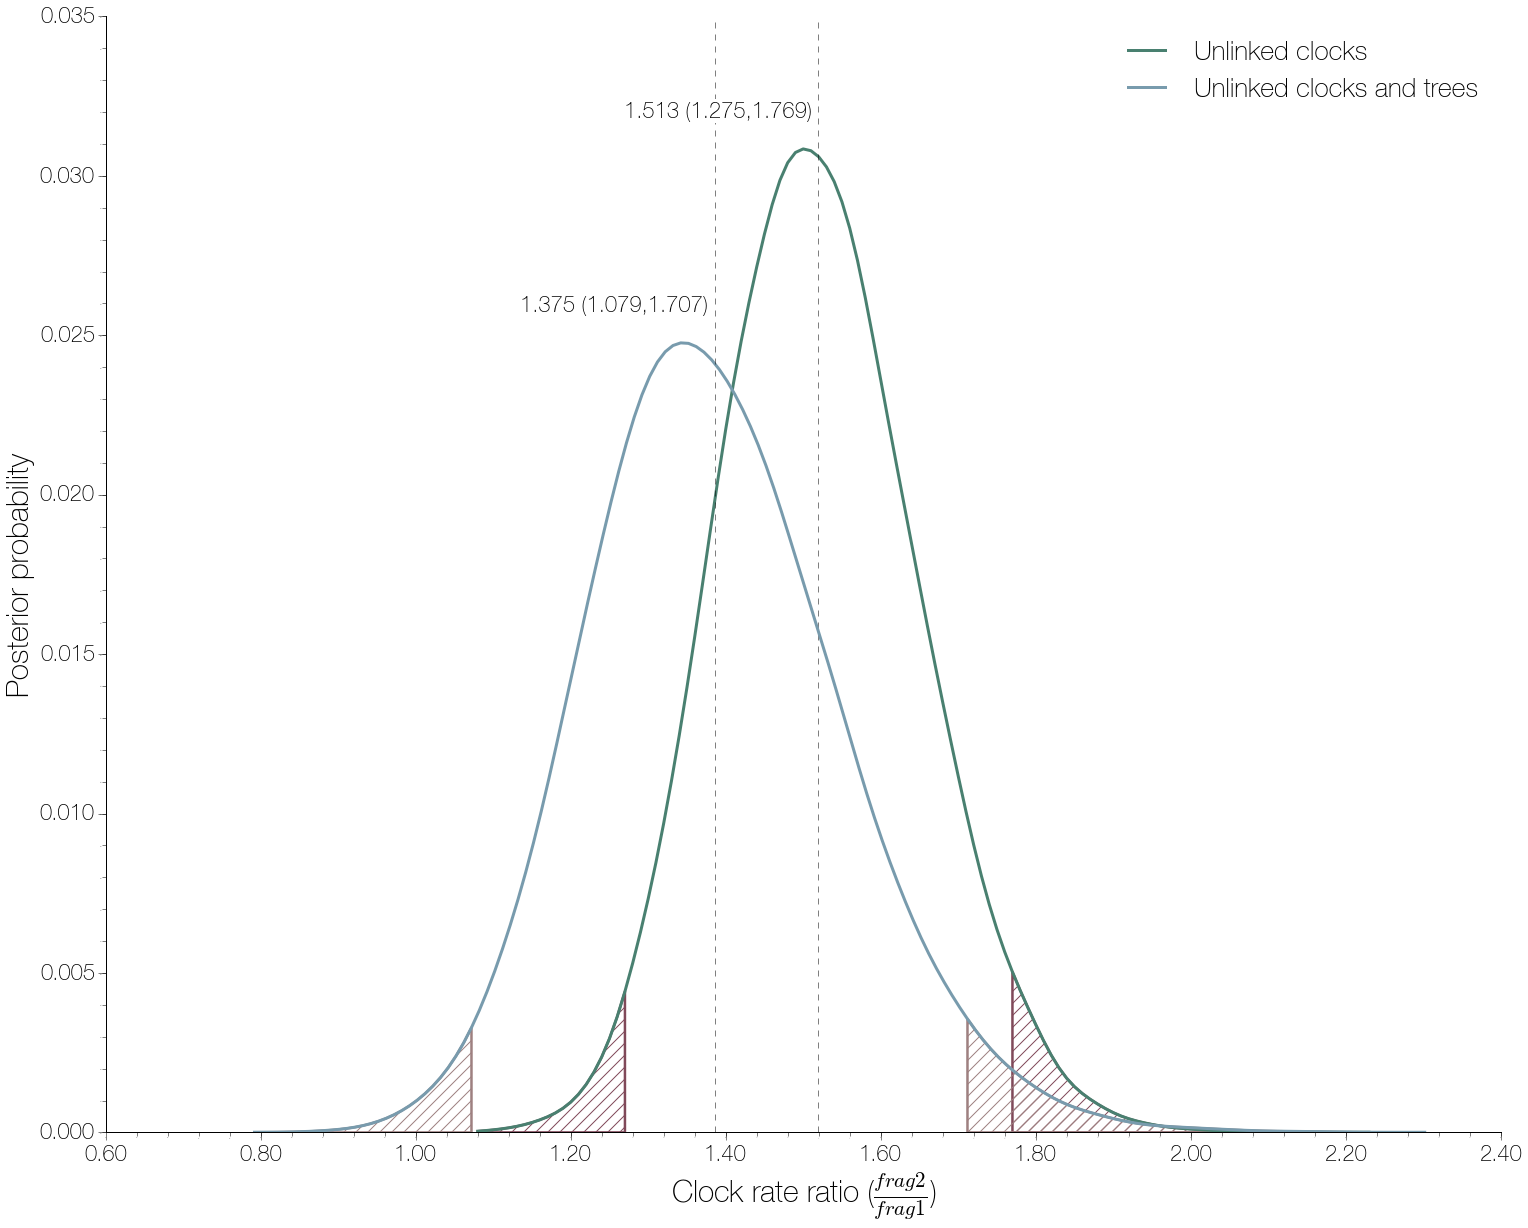
\includegraphics[width=0.8\textwidth]{figures/supp_MERS_empiricalHeterogeneity.png}
	\caption{\textbf{Empirical rate heterogeneity in MERS-CoV genome.}
Posterior estimates of the ratio between the molecular clock rates estimated independently from GARD-inferred fragment 2 (positions 23723-30126) and fragment 1 (positions 1-23722) under independent or linked tree models derived from 3 independent marginal likelihood analyses.
Dotted lines indicate the mean of the distribution and numbers next to the line show the median and the 95\% highest posterior density intervals.}
	\label{rateHet}
\end{figure}

%\subsection*{Permutation test results}

\begin{figure}[h]
	\centering	
	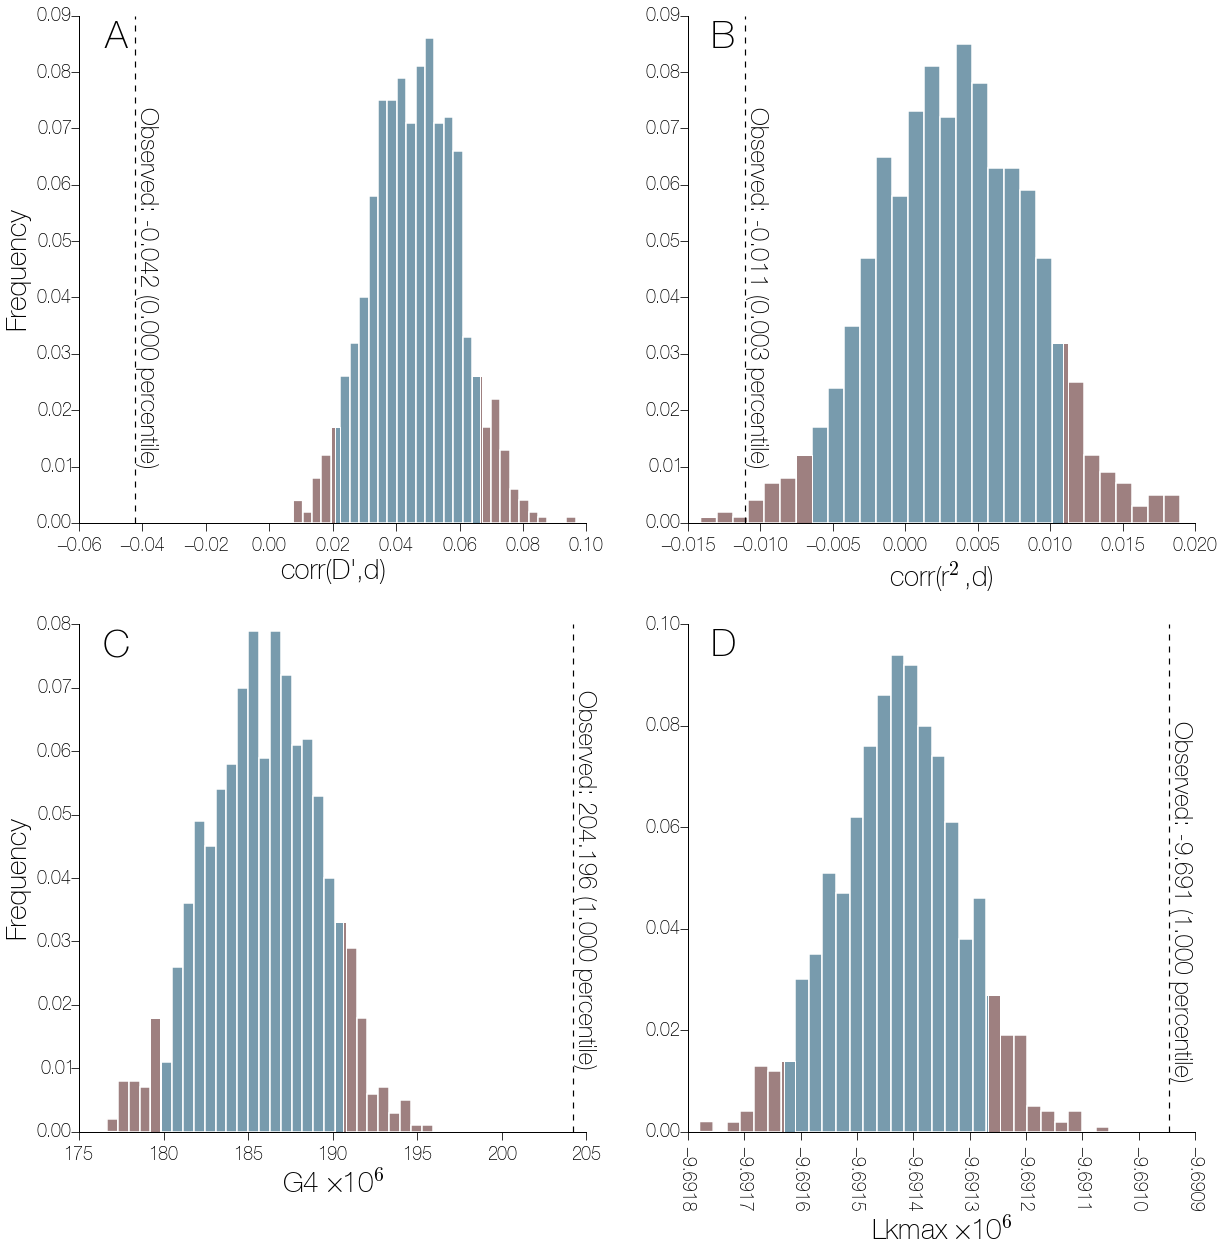
\includegraphics[width=0.75\textwidth]{figures/supp_MERS_permutations.png}
	\caption{\textbf{LDhat permutation test results for MERS-CoV.}
All 4 observed LD decay statistics (A - corr(D',d), B - corr(r$^{2}$,d), C - G4, D - Lkmax) for MERS-CoV data fall outside the distribution generated by permuting sites in ways consistent with recombination.}
	\label{MERS_permutations}
\end{figure}

%\subsection*{Composite likelihood methods are susceptible to rate heterogeneity}

\begin{figure}[h]
	\centering	
	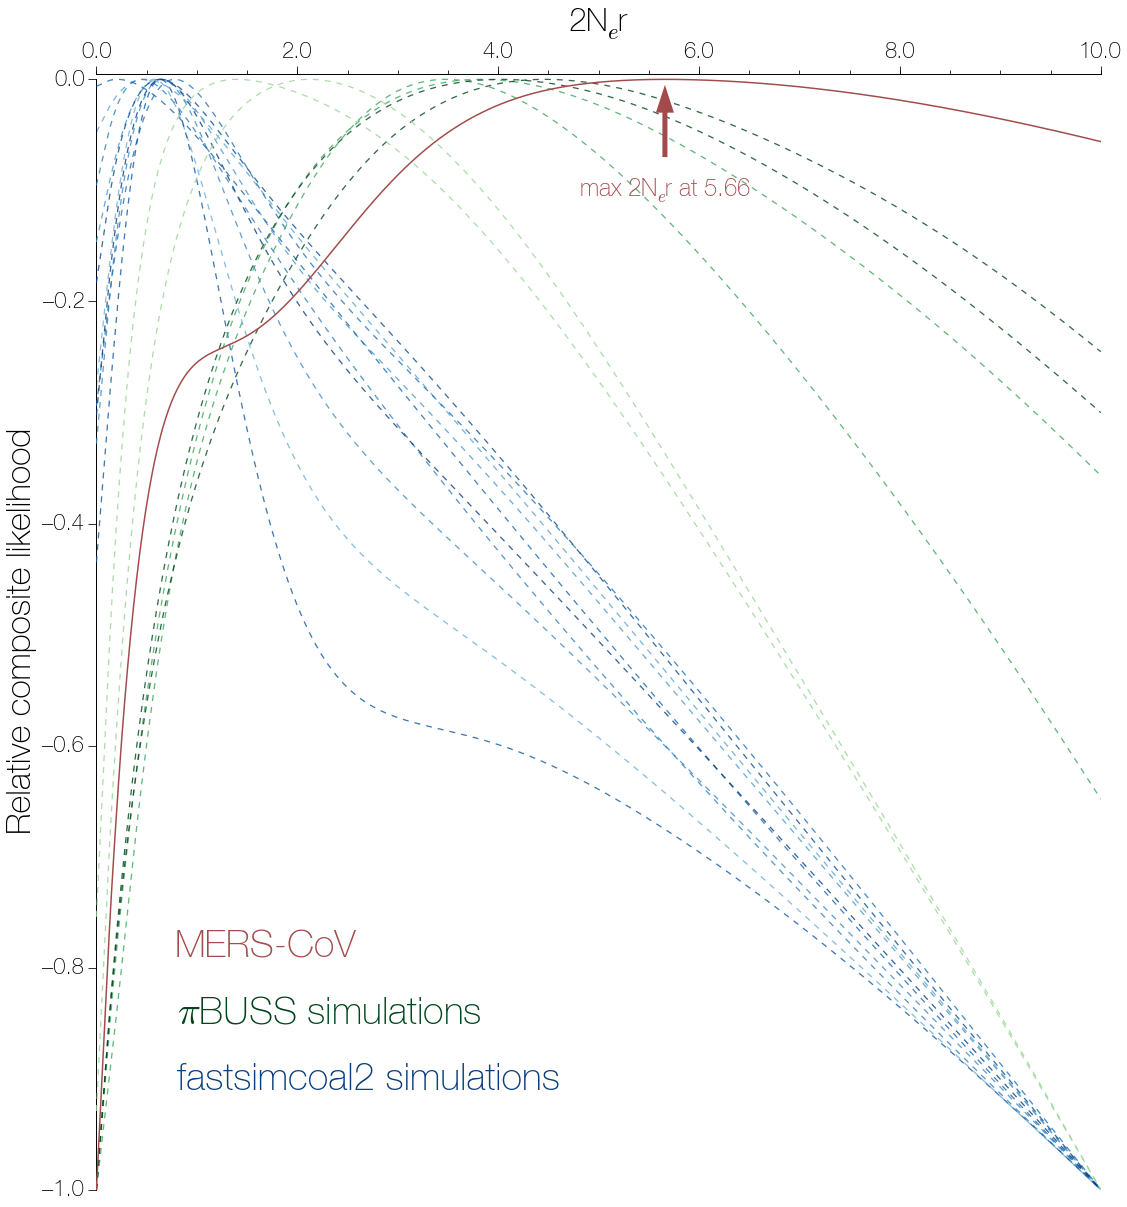
\includegraphics[width=0.6\textwidth]{figures/supp_MERS_compositeLikelihoods.png}
	\caption{\textbf{Relative composite likelihood surface.}
Composite likelihoods for the recombination rate estimates were rescaled to be within the range [-1,0].
Surfaces are coloured by data source: MERS-CoV estimate is in red, $\pi$BUSS simulations in green and fastsimcoal2 simulations in blue.
Colour scheme is identical to figure \ref{permutations} in the main text.
Maximum composite likelihood for MERS-CoV data is achieved at $\rho$=5.66, all other datasets have an inferred recombination rate above 0 despite being simulated without recombination.}
	\label{compLikelihoods}
\end{figure}

\begin{figure}[h]
	\centering	
	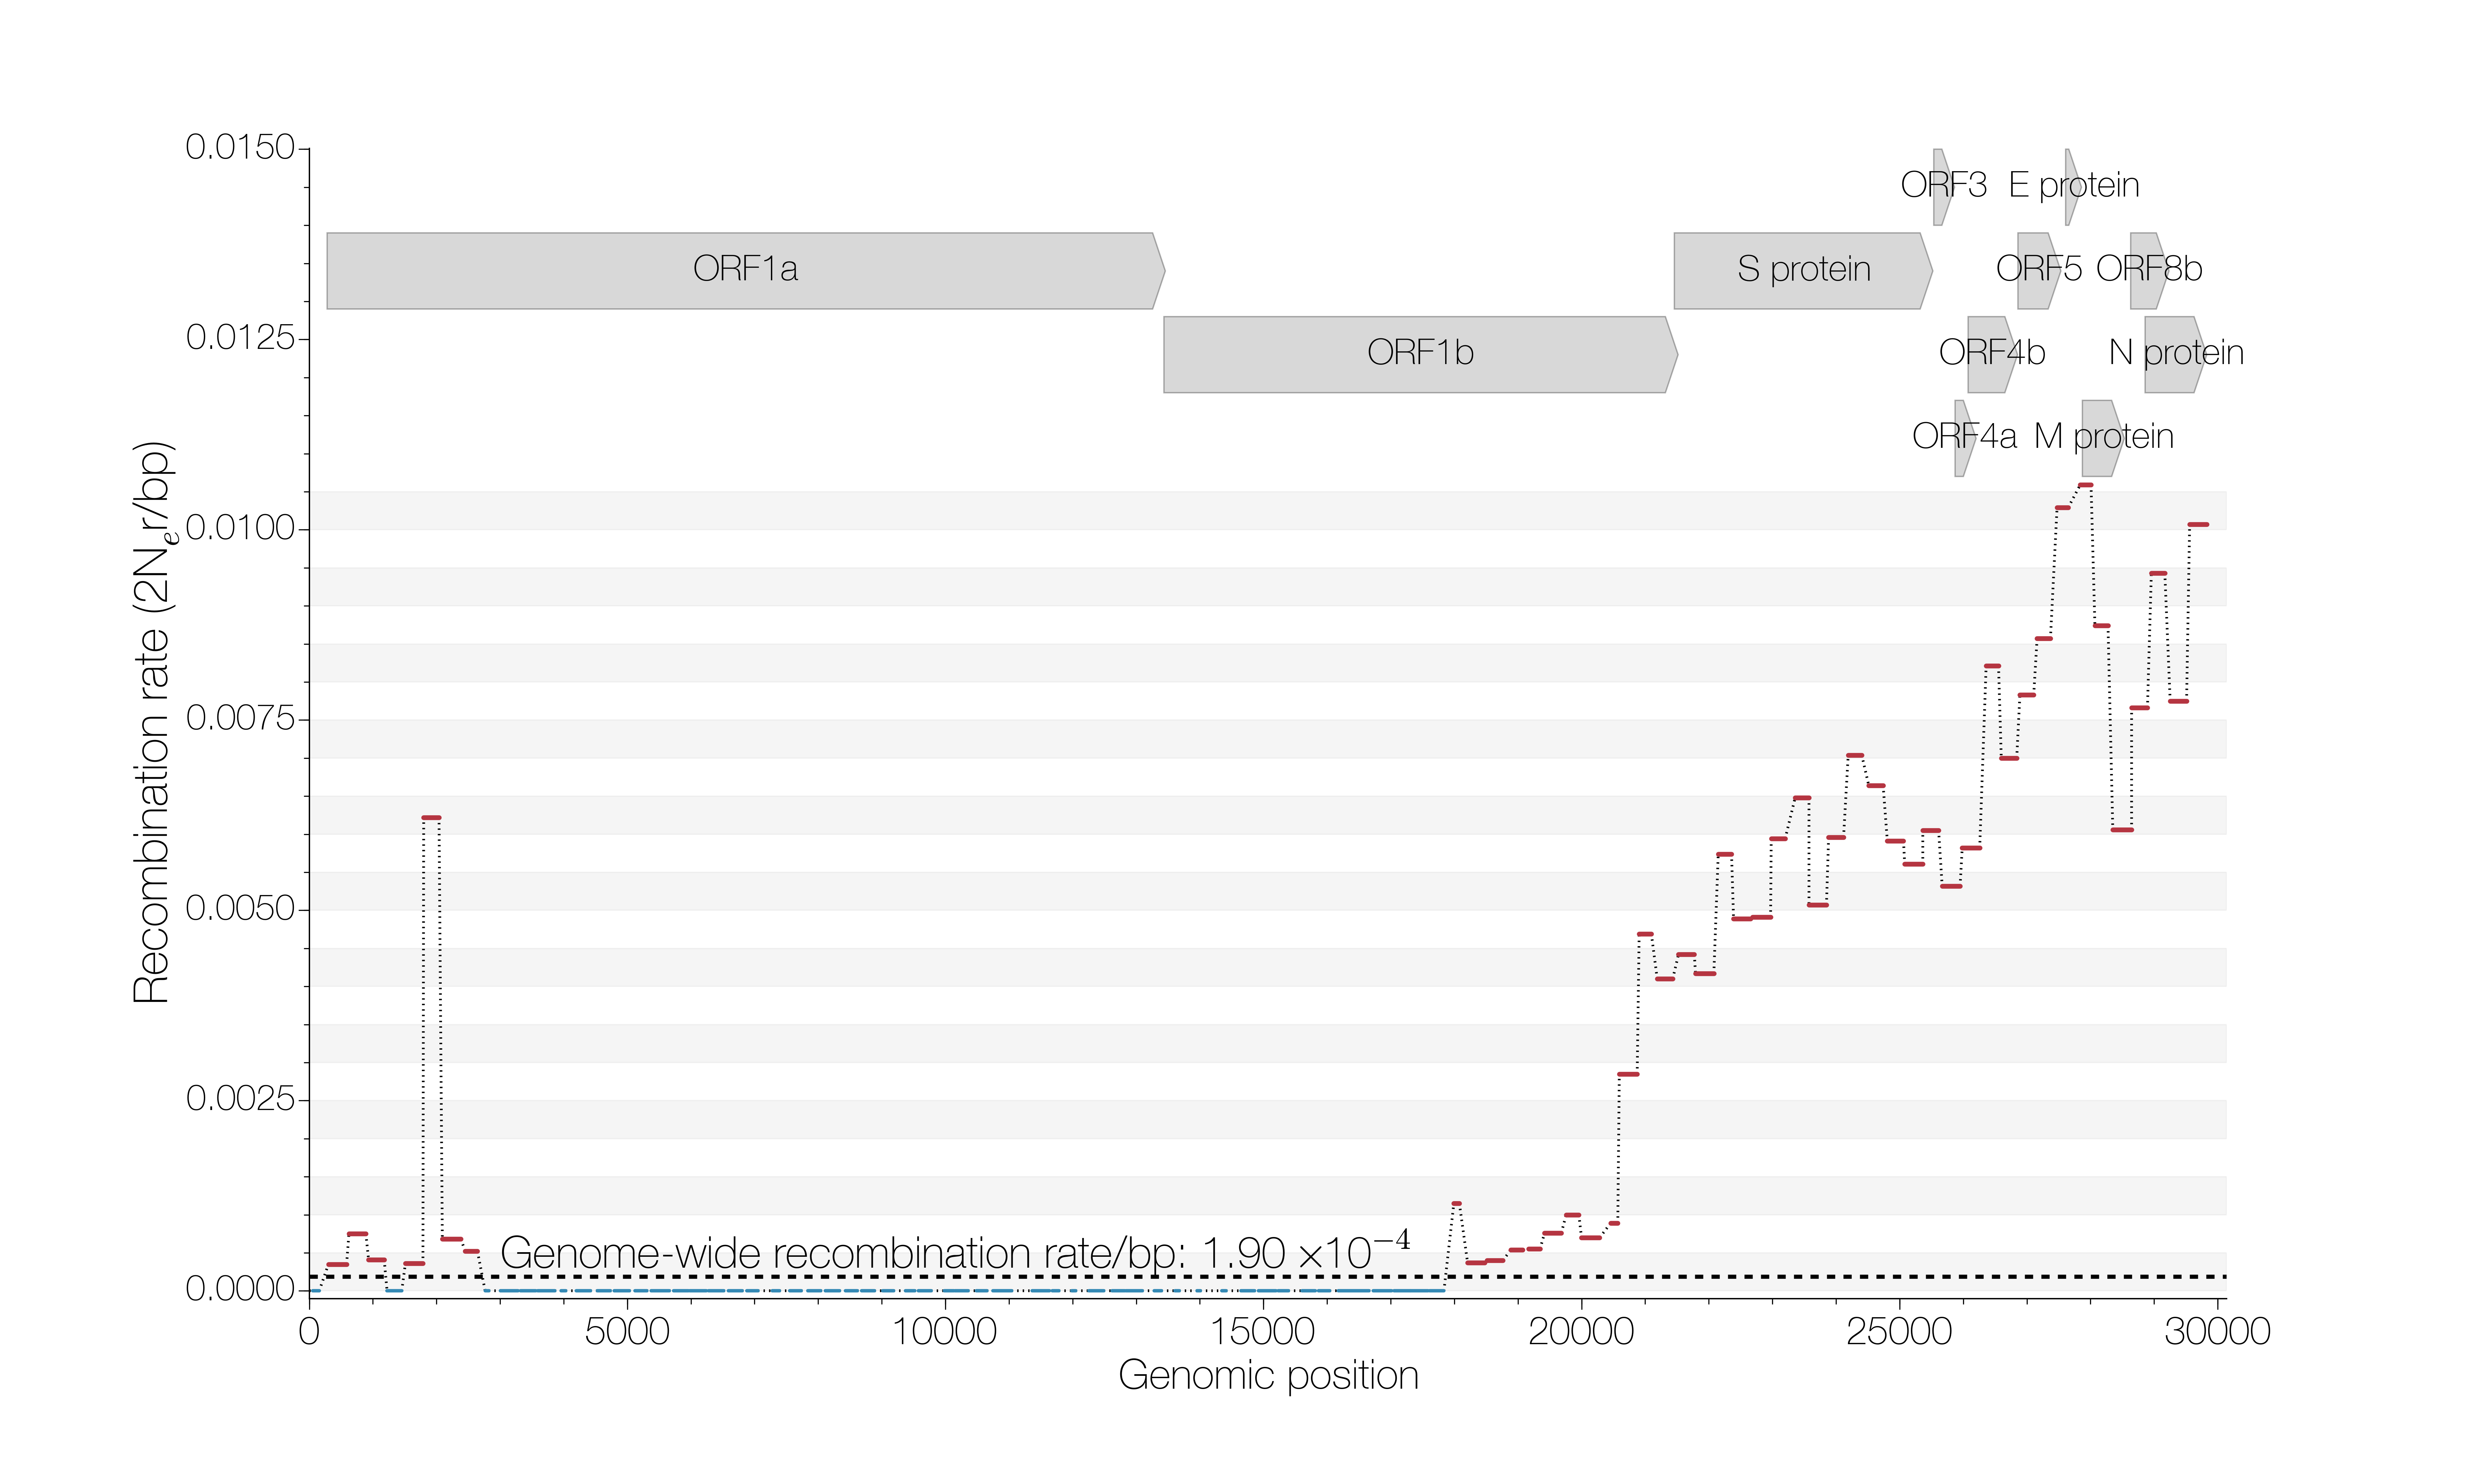
\includegraphics[width=0.7\textwidth]{figures/supp_MERS_LDhat_windowRho.png}
	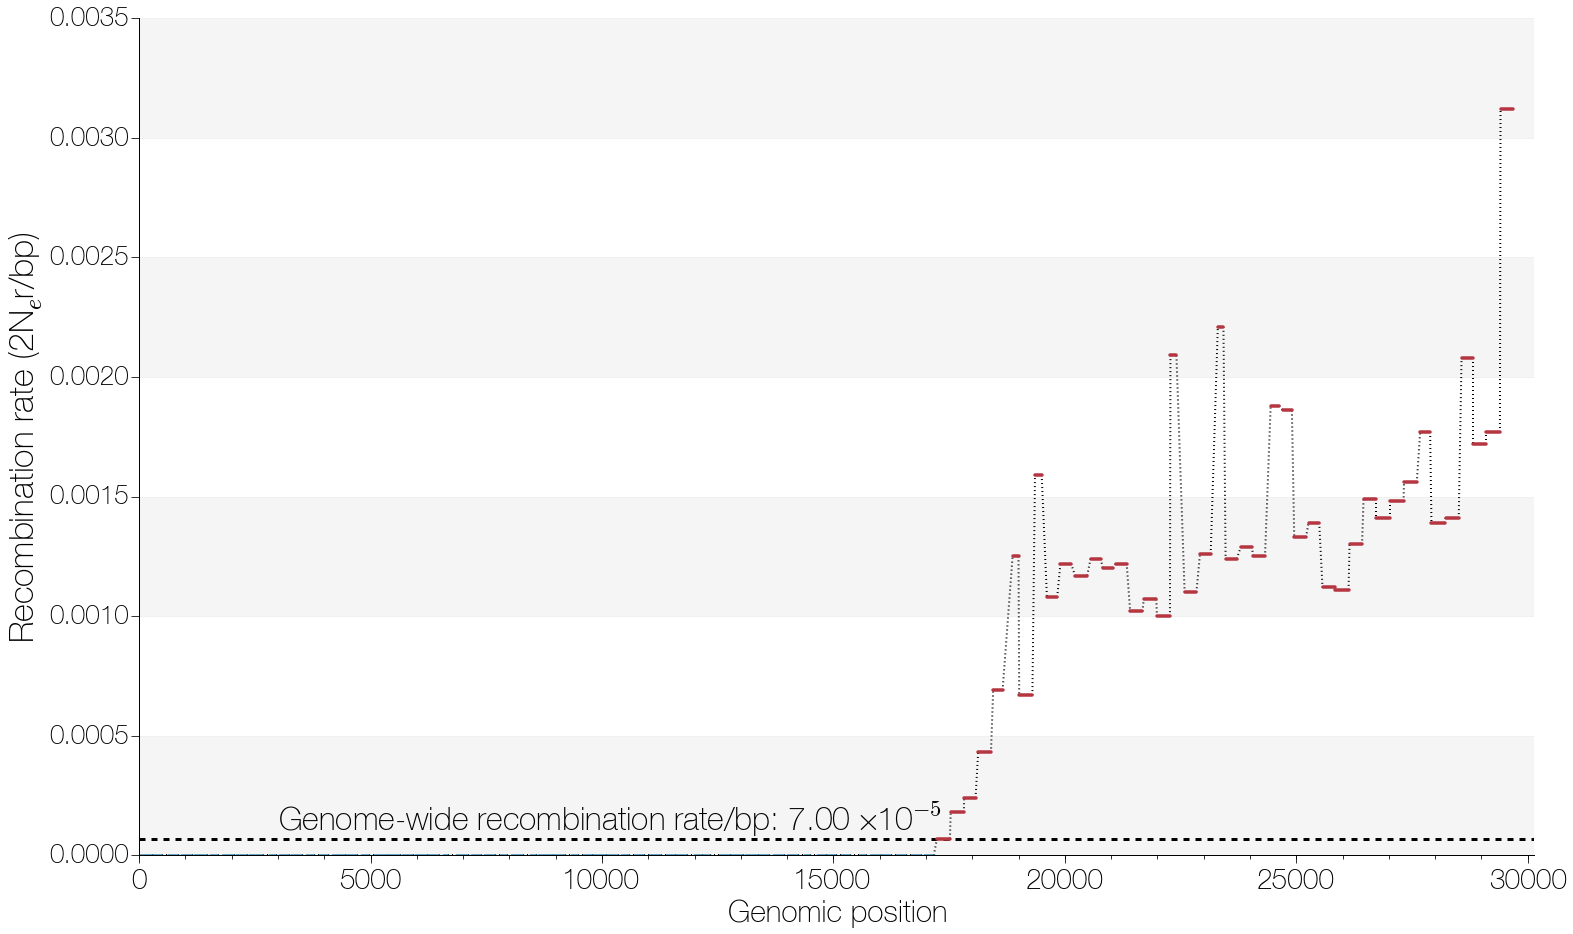
\includegraphics[width=0.7\textwidth]{figures/supp_pibuss1.3_LDhat_windowRho.png}
	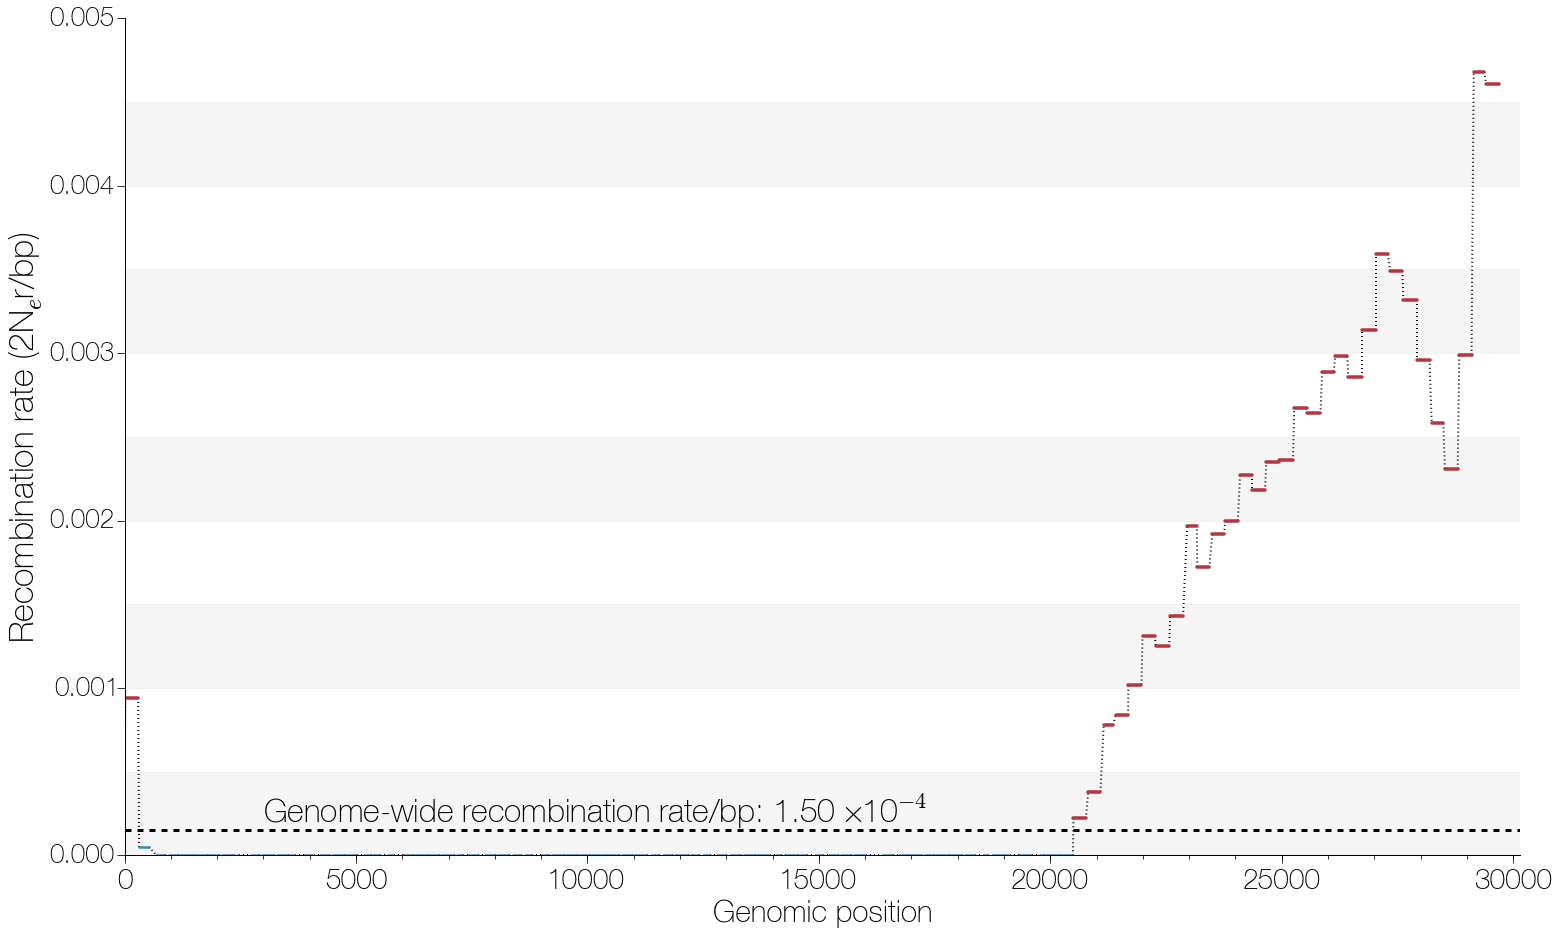
\includegraphics[width=0.7\textwidth]{figures/supp_pibuss3_LDhat_windowRho.png}
	\caption{\textbf{Window-based estimates of recombination rate.}
Inferred recombination rates for 300 nucleotide-long windows in MERS-CoV genome (top), $\pi$BUSS-simulated sequences with 1.3$\times$ rate heterogeneity (middle) and 3$\times$ rate heterogeneity (bottom).
Recombination rates that are above the inferred genome-wide recombination rate are in red.
Simulated rate heterogeneity is sufficient to mislead this method, although the inferred recombination rates in the last third of the MERS-CoV genome are much greater than those inferred from the simulated data.}
	\label{rho}
\end{figure}

\begin{figure}[h]
	\centering	
	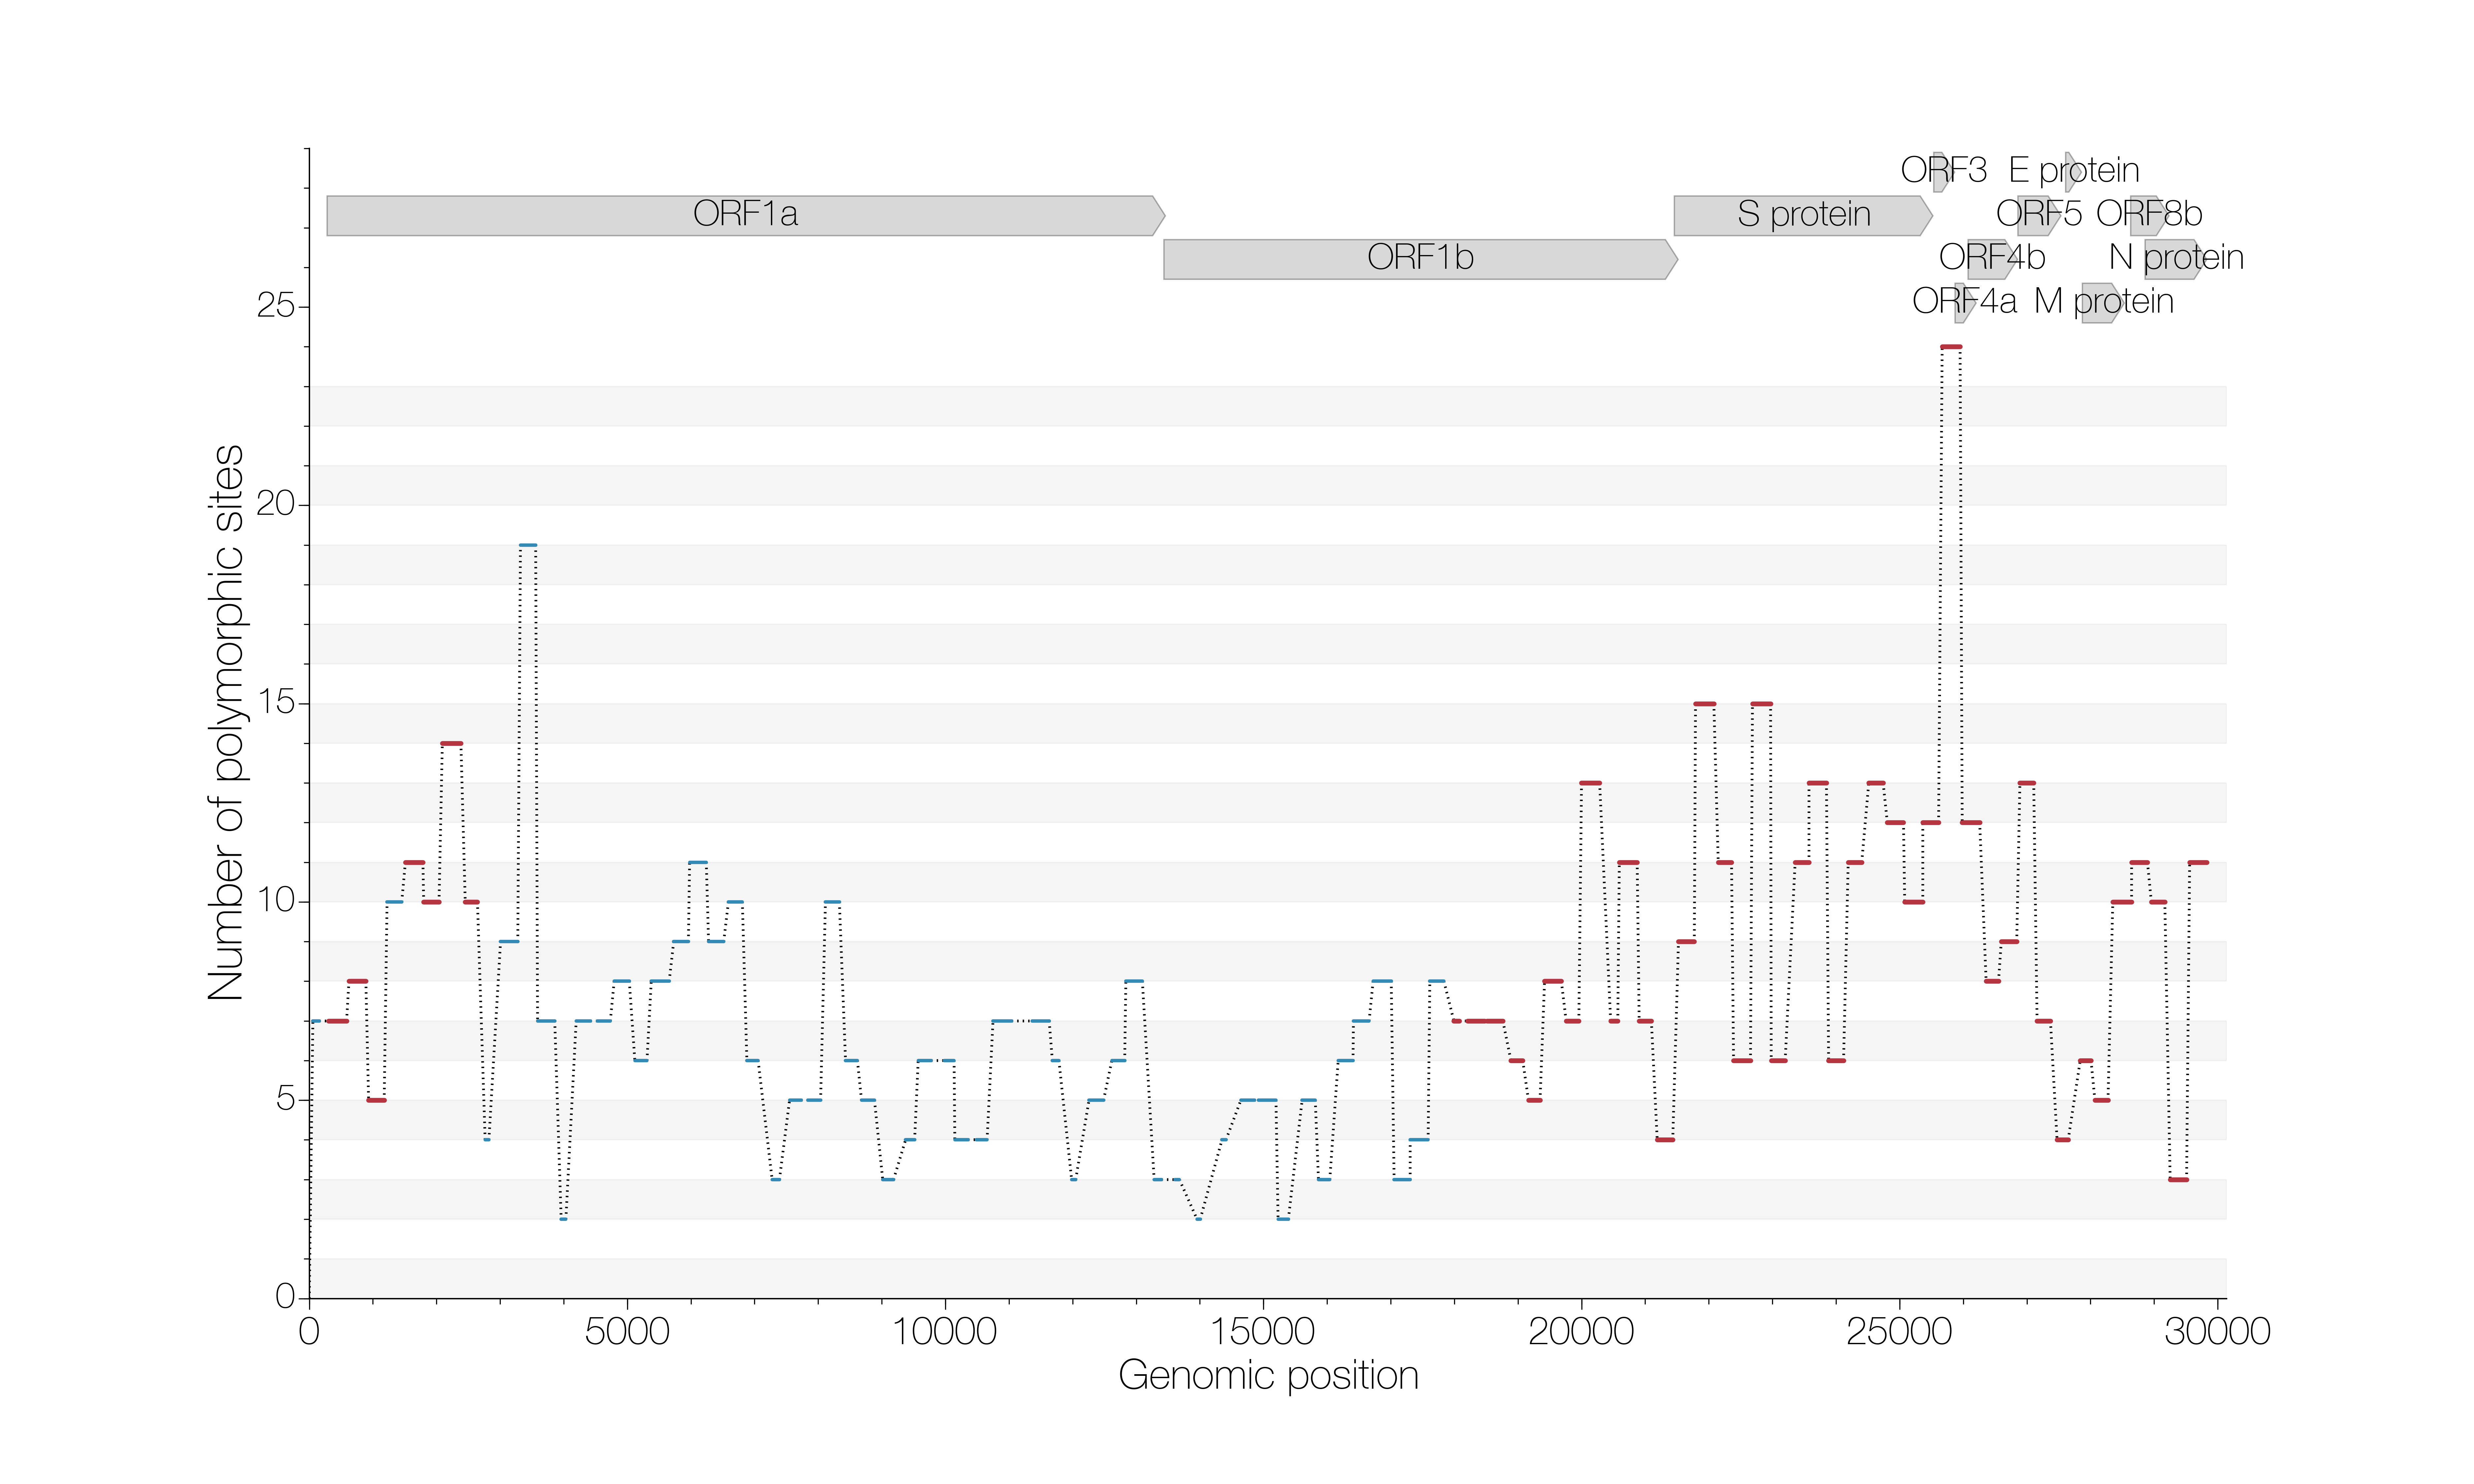
\includegraphics[width=0.7\textwidth]{figures/supp_MERS_LDhat_windowSNPs.png}
	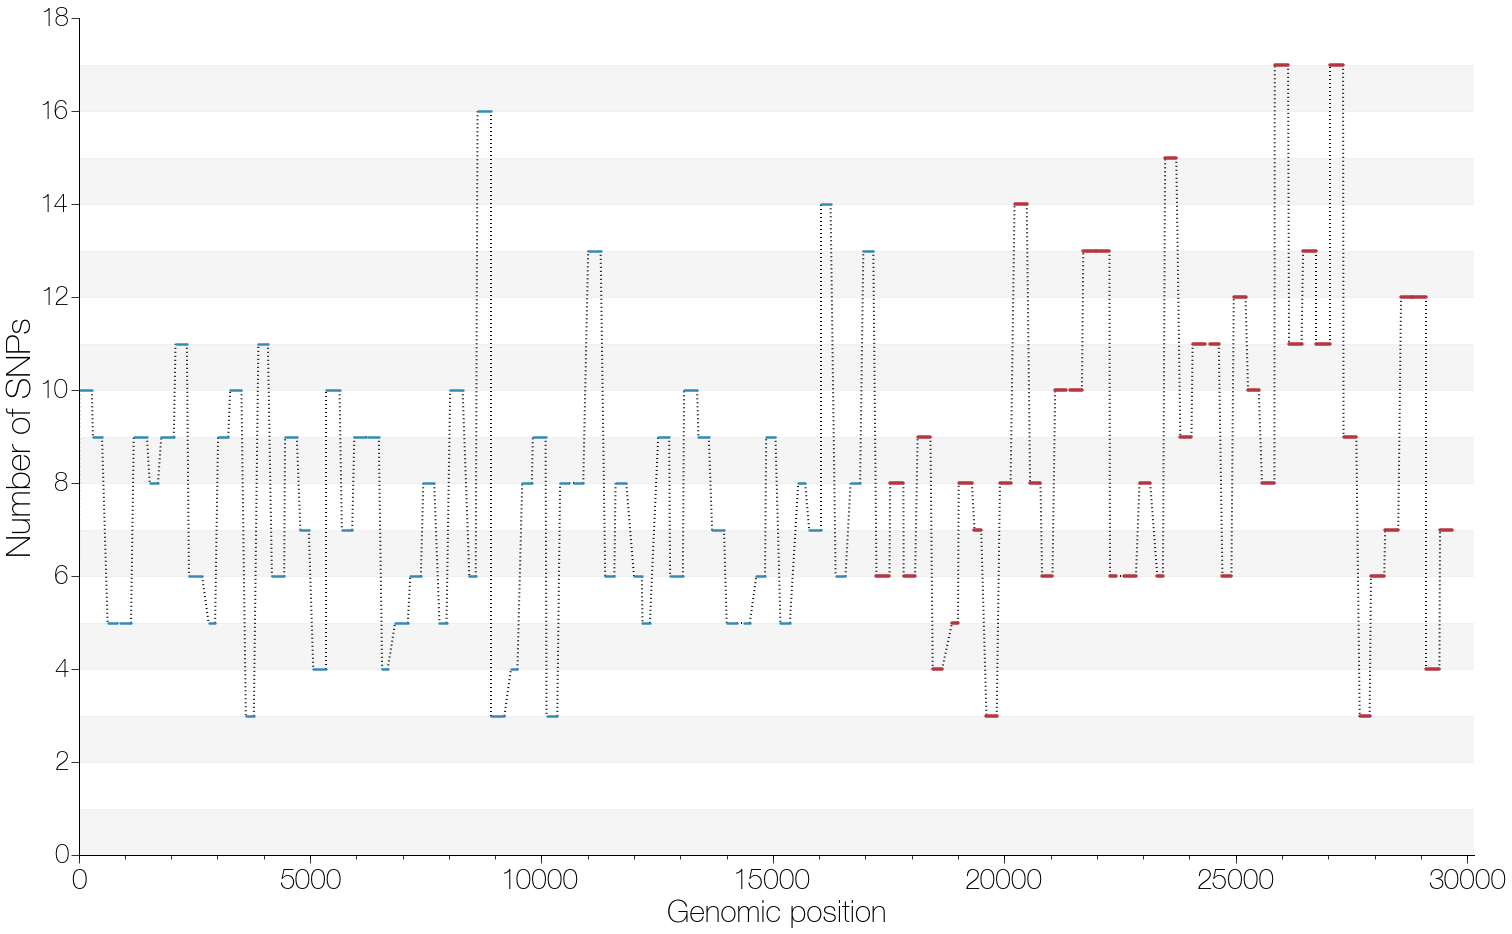
\includegraphics[width=0.7\textwidth]{figures/supp_pibuss1.3_LDhat_windowSNPs.png}
	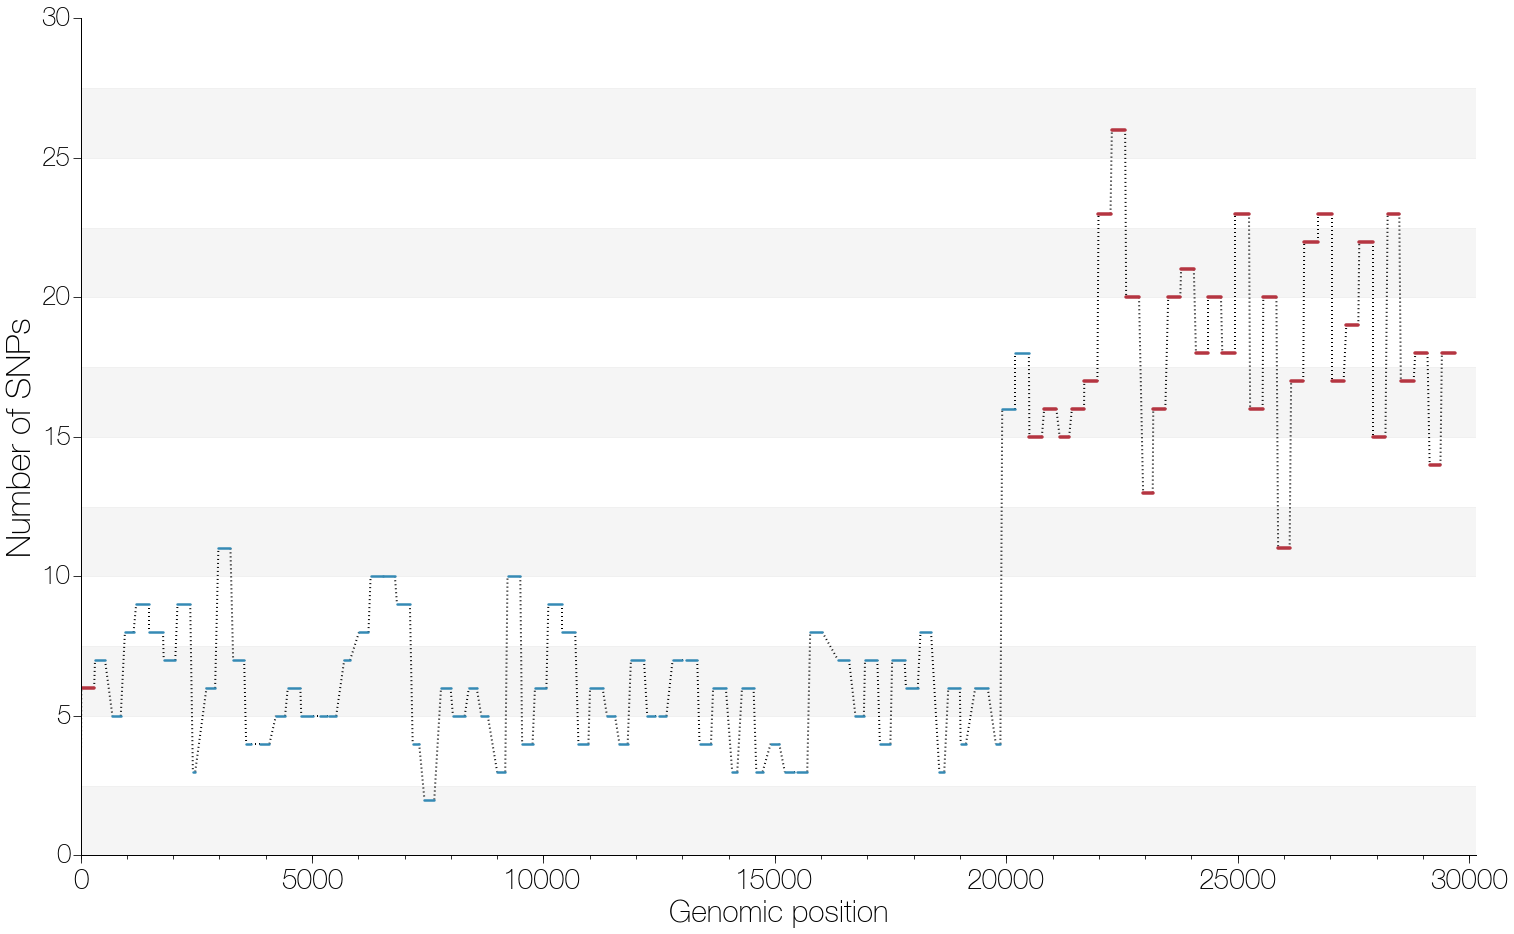
\includegraphics[width=0.7\textwidth]{figures/supp_pibuss3_LDhat_windowSNPs.png}
	\caption{\textbf{Window-based estimates of polymorphic site density.}
Inferred polymorphic site densities for 300 nucleotide-long windows in MERS-CoV genome (top), $\pi$BUSS-simulated sequences with 1.3$\times$ rate heterogeneity (middle) and 3$\times$ rate heterogeneity (bottom).
Windows are coloured red if their recombination rate is above the inferred genome-wide recombination rate.
Extreme rate heterogeneity (3$\times$) results in a higher density of polymorphic sites in the region with the higher rate.}
	\label{SNPs}
\end{figure}

%\subsection*{Bayesian ancestral sequence reconstruction agrees with ML methods}

\begin{figure}[h]
	\centering	
	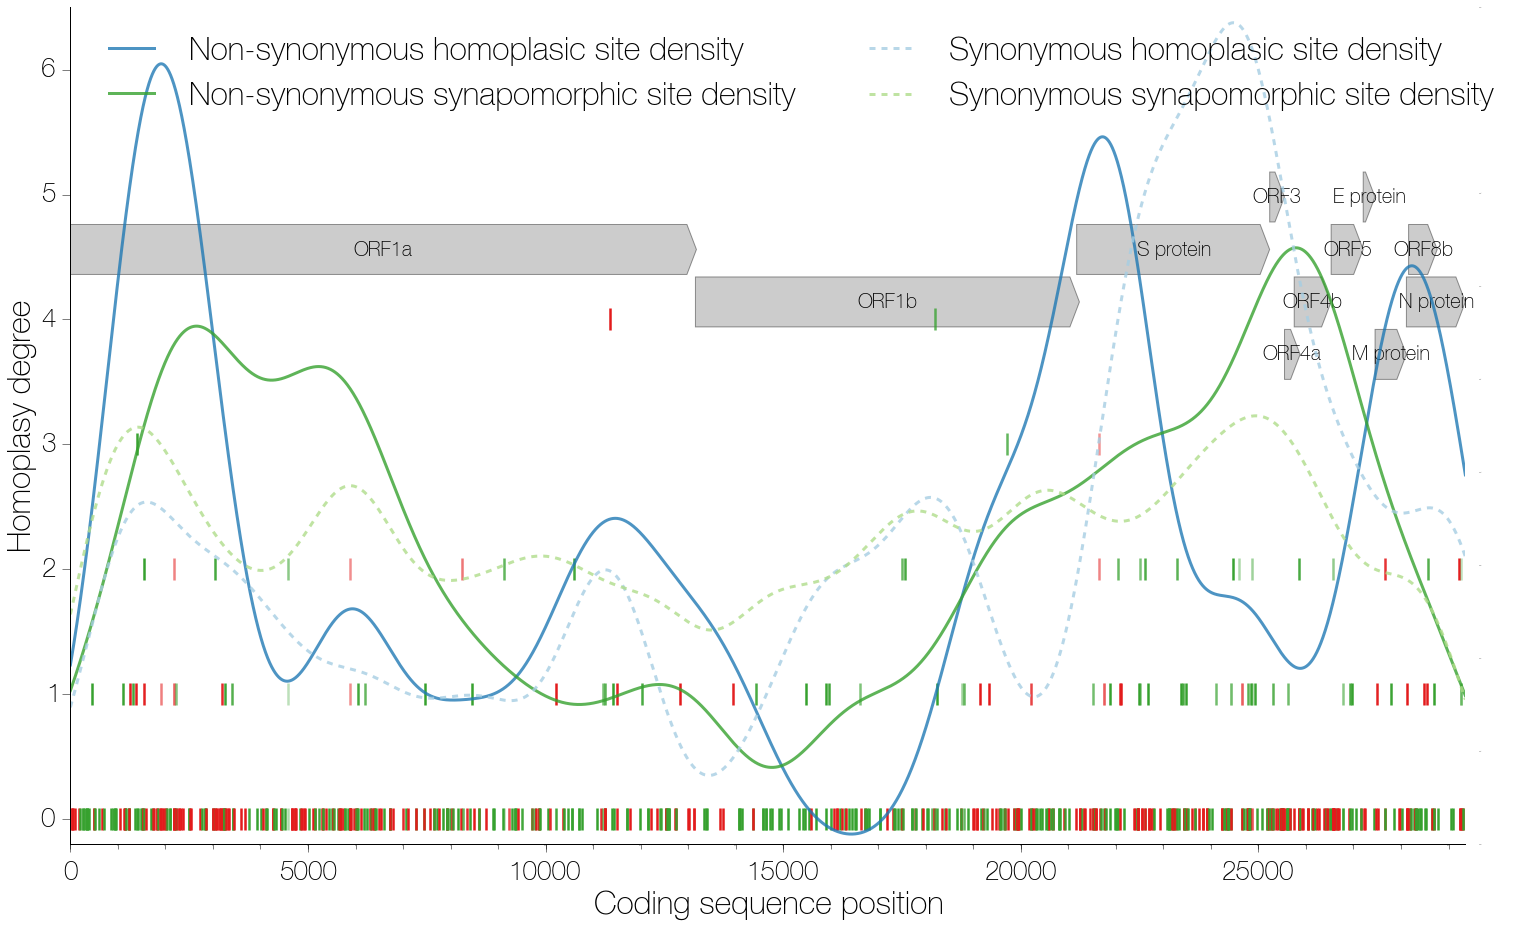
\includegraphics[width=0.85\textwidth]{figures/supp_MERS_BEAST_homoplasyRate.png}
	\caption{\textbf{Homoplasy degrees inferred by BEAST.}
Position along the genome is shown on the x axis and homoplasy degree, the number of times a particular mutation has occured in excess in the tree, is shown on the y axis.
Individual mutations are marked by vertical lines, synonymous ones in green and non-synonymous in red with transparency representing the posterior probability of a given homoplasy degree for each mutation.
Kernel density estimates of homoplasic/synapomorphic and synonymous/non-synonymous sites are shown as blue and green lines.
Arrows at the top indicate the positions and names of coding sequences within the MERS-CoV genome.}
	\label{homoplasyRates_Bayesian}
\end{figure}


%\subsection*{Host association}

\begin{figure}[h]
	\centering	
	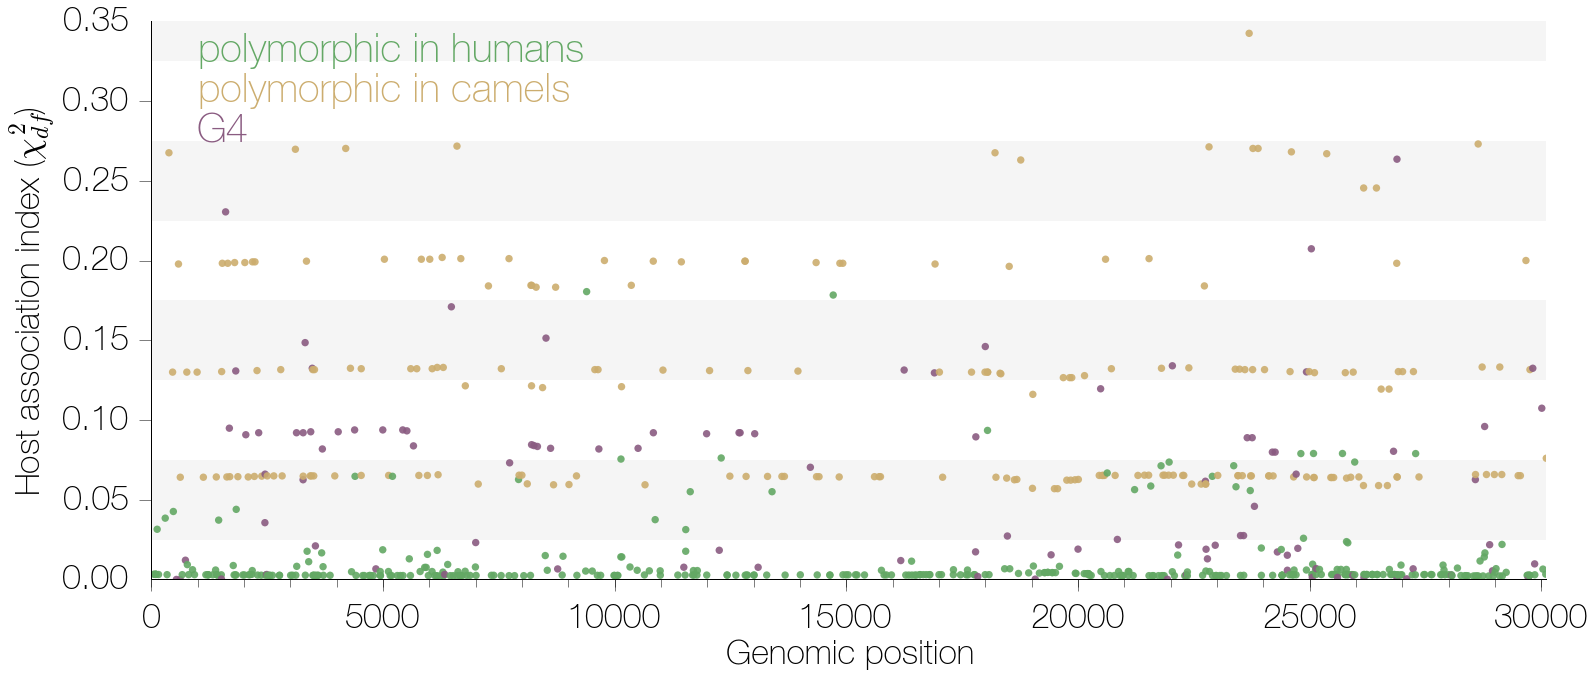
\includegraphics[width=0.85\textwidth]{figures/supp_MERS_hostAssociation.png}
	\caption{\textbf{Host association indices for variable sites.}
Estimates for the association between particular alleles and host.
The association index is an adapted version of the $\chi^{2}_{df}$ statistic of LD, and quantifies how well one can predict the allele at any given polymorphic site, given the host it was isolated from.
No perfect associations (association index = 1.0) between particular alleles and host (human or camel) were found.}
	\label{host_association}
\end{figure}

\clearpage

%\bibliographystyle{mbe}
%\bibliography{MERS_rec}

\end{document}